\documentclass[a4paper]{article}
% \documentclass{llncs}
\usepackage[english]{babel} \usepackage[colorlinks=true]{hyperref} \usepackage{float}
\usepackage[utf8]{inputenc} \usepackage{amsmath} \usepackage{graphicx}
\usepackage[colorinlistoftodos]{todonotes} \usepackage{tikz}
\usepackage{pdfpages} \usepackage{listings}
\usepackage{listings}
\usepackage{color}
\usepackage{framed,enumitem}
\usepackage{float}
\usepackage{subcaption}
\usepackage{amsthm}
\usepackage{biblatex}


\addbibresource{references.bib}

\newtheorem{theorem}{Theorem}[section]
\newtheorem{corollary}{Corollary}[theorem]
\newtheorem{lemma}[theorem]{Lemma}

\definecolor{green}{rgb}{0,0.6,0}
\definecolor{gray}{rgb}{0.5,0.5,0.5}
\definecolor{mauve}{rgb}{0.58,0,0.82}

\lstset{frame=tb,
  language=Java,
  aboveskip=3mm,
  belowskip=3mm,
  showstringspaces=false,
  columns=flexible,
  basicstyle={\small\ttfamily},
  numbers=left,
  numberstyle=\tiny\color{gray},
  commentstyle=\color{green},
  stringstyle=\color{mauve},
  breaklines=true,
  breakatwhitespace=true,
  tabsize=3
}
% add above keywordstyle=\color{blue},

\lstset{emph={%  
    for%
    },emphstyle={\color{blue}\bfseries}%
}%

\lstset{escapeinside={(*@}{@*)}}

\renewcommand{\lstlistingname}{Algorithm}

\usetikzlibrary{arrows,positioning,shapes.geometric}



\title{A* for Dynamic Graphs on GPU}



\author{\normalsize Lokesh Koshale (CS15B049)\normalsize}
% \institute{CS15B049}
\date{}


\begin{document} \maketitle


% \section{Abstract}
%  We propose algorithm and techniques to solve the dynamic A star guided search on GPU.
% The goal of a dynamic graph algorithm is to
% support query and update operations as
% quickly as possible.

% In many applications graphs are subject to discrete changes, such as additions or deletions
% of edges or vertices.

% The goal of
% a dynamic graph algorithm is to update efficiently the solution of a problem after dynamic changes,
% rather than having to recompute it from scratch each time

\section{Introduction}\label{sec:introduction}
A*~\cite{A*,wiki_a_star} is one of the widely used path planning and shortest path approximation algorithms. It is used in several applications due to its performance and accuracy. A* is applied in a diverse set of problems from path-finding in video games and robotics to codon optimization in genetics. In several real-life graph applications such as wireless networks, the underlying graph is not static but is evolving. D*~\cite{original_D_star, wiki_d_star}, focused D*~\cite{focused_D_star}, and D* lite~\cite{D_star_lite} form a family of informed incremental search algorithms where edge cost can change while the optimal path is being explored. In this work, we focus on A* for graphs that are subjected to update operation, where an update operation refers to the insertion or deletion of an edge. Instead of performing A* again from start each time graph is subject to update, our algorithm process the sub-graphs which are affected by the update. Compared to repeated A* our algorithm performs better and we have observed an increase in speedup which is proportional to the number of updates the graph is subjected to. For temporal graph available at SNAP~\cite{SNAP} for 100 updates we got 25$\times$--40$\times$ of performance improvement over repeated A* search. A* has various applications and one of them is in energy-efficient routing for wireless sensor networks, where the graph is inherently dynamic in nature. One of such routing algorithm is EERP~\cite{WSN2014} we have done a comparison between EERP with native A* and EERP with our algorithm, We got 24$\times$--55$\times$ performance improvement by using our algorithm.
\\
% \todo{Mention our results on synthetic graphs and also the application.}
In this document section~\ref{sec:background} explains A* algorithm and how it is implemented for GPU. Section~\ref{sec:incremental} discusses how insertions are processed in parallel to find the optimal path. Section~\ref{sec:decremental} explains the implications deletion on the optimal path and also reasons why deletion in the cyclic graph requires additional checks. Section~\ref{sec:fully_dynamic} presents methods for processing insertion and deletion combined together and contains the proof of correctness of our algorithm. Section~\ref{sec:experiments} contains a detailed analysis of experiments performed and its results. Section~\ref{sec:applications} shows how our algorithm can be used to improve performance in various applications that uses A*.

% \todo{Mention outline of this report: Section~\ref{sec:background} explains A* algorithm. ...}

\section{Background}\label{sec:background}
In this section we discuss A* and its GPU implementation in detail.
Algorithm~\ref{algo:a_star} A* takes a Graph with source node(start) and destination node(end) as input and returns the optimal path from source to the destination node. We initialize open\_list which is a priority queue with start node(Line 5). As cost of reaching source from source is 0, $g(start)$ is set to 0 (Line 7),Then we compute the heuristics\_function (Line 8) from start to end which is the approximate cost of reaching destination from source and then use it compute $f(start)$(Line 9). While open\_list is not empty we extract a node with the minimum cost from it(Line 12), Then we check if the extracted node is the destination node, if it is then we return the path(Line 14). Otherwise, we add this node to closed\_list(Line 15). Then we compute the cost of reaching the child from the source through this parent i.e $g$ value for each of its children(Line 18-19). If the newly computed cost is less than old cost i.e $g(child)$ and the node is present in either list we remove the node from the list( Line 21-25 ). Then if the child is not present at either list we compute the $f(child)$ with new cost and add it to the open\_list (Line 27-31). If we exhaust all nodes and haven't found the destination node we return failure(Line 33) as there is no path from source to destination.

% \todo{Let us refer to the algorithm and explain it using line numbers.}

\begin{lstlisting}[language=C , caption=A*~\cite{A*},label={algo:a_star} ]
Input: A Graph(V, E) with source node (*@\textit{start}@*) and goal node (*@\textit{end}@*).
Output: Least cost path from (*@\textit{start}@*) to (*@\textit{end}@*).
Steps:
Initialize 
    open_list = {(*@\textit{start}@*)}          /* list of nodes to be traversed */
    closed_list = {}              /* list of already traversed node */
    g(start) = 0                  /* cost from source node to node */
    h(start) = heuristic_function(start,end) /* estimated cost from source to goal node */
    f(start) = g(start) + h(start)      /* total cost from goal to node */
    
    while open_list is not empty:
        m = node on top of open_list with least f
        if m == end
            return
        remove m from open_list
        add m to close list
        
        for each n in child(m):
            cost = g(m) + distance(m,n)
            
            if n (*@$\in$@*) open_list and cost < g(n):
                remove n from open_list     /* new path is better */
                
            if n (*@$\in$@*) closed_list and cost < g(n):
                remove n from closed_list
                
            if n (*@$\notin$@*) open_list and n (*@$\notin$@*) closed_list:
                g(n) = cost
                h(n) = heuristic_function(n, end)
                f(n) = g(n) + h(n)
                add n to open_list
    
    return failure
    
\end{lstlisting}

General-purpose computation on graphics processing units (GP-GPU) has been widely used to accelerate numerous computational tasks. In multi-core systems to improve the performance, one has to increase the number of cores and adding more and more cores increases the cost thus GPU is cost-efficient alternative hardware to execute parallel algorithms which also provides better performance. Zhou and Zeng~\cite{GA*} proposed a parallel variant of A* for GPU. We borrow the parallelization of A* on GPU from them. The bottleneck for parallelization is the sequential nature of Priority Queue which is the primary data structure to implement A*, to utilize the many-core GPU architecture the authors proposed to have multiple priority queues thus expanding many nodes at once. In the paper, the authors claim that GA* achieves 30$\times$--45$\times$ performance improvement from the CPU implementation.\\
Algorithm~\ref{algo:ga_star} describes the framework of GA* algorithm using parallel priority queues. For each state s in the open\_list or closed\_list, $s.node$ stands for the last node in the path represented by $s$, $s.f$ and $s.g$ store the values of $f(s)$ and $g(s)$, respectively, and $s.prev$ stores the pointer to the previous state that expanded $s$, which is used to regenerate a path from a given state. List S stores the expanded nodes and list T stores the nodes after the removal of duplicated nodes. Lines 24-29 detect the duplicated nodes, where $H[n]$ represents the state in the closed list in which the last node in its path is node $n$. Through synchronization operations, which are computationally cheap on GPUs, we can push nodes expanded from the same parent into different queues (Line 32), as nodes with the same parent tend to have similar priority values.

% \todo{Let us refer to the algorithm and explain it using line numbers.}

\begin{lstlisting}[language=FORTRAN, caption=GA*~\cite{GA*},label={algo:ga_star}]
procedure GA*(s, t, k)   !find the shortest path from s to t with k queues
Let (*@$\{Q_i\}^k_{i=1} $@*) be the priority queues of open_list
Let H be the closed_list
PUSH((*@$Q_1$@*), s)
m (*@$\leftarrow$@*) nil         !m stores the best target state
while (*@$Q$@*) is not empty do:
    Let (*@$S$@*) be an empty list
    for i (*@$\leftarrow$@*) 1 to k in parallel do:
        if (*@$Q_i$@*) is empty then
            continue
        end if
        (*@$q_i \leftarrow$@*) Extract((*@$Q_i$@*))
        if (*@$q_i.node = t$@*) then:
            if m = nil or (*@$f(q_i) < f(m)$@*) then:
                m (*@$\leftarrow q_i$@*)
            end if
            continue
        end if
        (*@$S \leftarrow S + EXPAND(q_i)$@*)
    end for
    if m (*@$\neq$@*) nil and (*@$f(m) \leq min_{q\in Q}f(q)$@*) then:
        return the path generated from m
    end if
    (*@$T \leftarrow S$@*)
    for (*@$s'\in S$@*) in parallel do:
        if (*@$s'.node \in H$ @*) and (*@$H[s'.node].g < s'.g$@*) then:
            remove (*@$s'$@*) from (*@$T$@*)
        end if
    end for
    for (*@$t' \in T$@*) in parallel do:
        (*@$t'.f \leftarrow f(t')$@*)
        PUSH (*@$t'$@*) to one of priority queues
        (*@$H[t'.node] \leftarrow t'$@*)
    end for
end while
end procedure

\end{lstlisting}
Below are some terminology we will be using in this document.
\subsection{Terminology}
\begin{itemize}
    \item $g(n)$: cost of reaching node $n$ from source
    \item $h(n)$: approximate cost of reaching destination from node $n$
    \item $f(n)$: approximate cost of reaching destination from source via node $n$ $f(n) = g(n) + h(n)$
    \item $w_{uv}$: weight associated with the edge $u \rightarrow v$
    \item open\_list : list of nodes to be traversed.
    \item update\_list: list of nodes to be traversed while performing propagation for insertion/deletion of edges.
    \item optimal\_cost: same as $f(n)$
    \item optimal\_parent: back edge to the parent from which optimal cost is calculated
    \item Optimal\_Path: source to destination optimal path, which can be traced by following optimal\_parent from destination
    \item $f(n)_{old}$: approximate cost of reaching destination from source via node $n$ before updates (insertion/deletion)
    \item $f(n)_{new}$: approximate cost of reaching destination from source via node $n$ after updates (insertion/deletion)
\end{itemize}
We make certain claims regarding the state of the graph and prove them, which will be later useful in deriving some major algorithmic choices for processing addition and deletion of edges.

\begin{lemma}\label{lemma:Astar property}
If we have found a node $d$ which has cost $f_d$ then all the nodes $i \in V$ which have cost $f_i < f_d$ are already visited(expanded).
\end{lemma}
\begin{proof}
Suppose we found the node $d$ with cost $f_d$ and there exists a node n such that node $n$ is not visited i.e $n \notin closed\_list$ and $f_n < f_d$.\\
If $n \notin closed\_list$ then either node $n \in open\_list$ or $n$ is not explored yet which means $f_n = \infty $.
\begin{itemize}[label={}]
    \item  If $n \in open\_list$  and we know that $f_n < f_d$, In A* to expand a node we always chose the node with least $f$ ( as in line no 15 of Algorithm~\cite{algo:a_star}:A*).So $n$ should be chosen before $d$ and which implies that $n$ is already visited(expanded). which contradicts our assumption that $n$ is not visited.
    \item If $f_n = \infty $, we have found the node $d$ so $f_d \neq \infty$ which implies $f_n > f_d$ which contradicts our assumption that $f_n <  f_d$
\end{itemize}
hence proved.
\end{proof}

\begin{corollary}\label{corollary:Astar property}
If some nodes are not visited at the end of A* then those nodes will have cost greater than or equal to the cost of destination. 
\end{corollary}


\section{Incremental Processing}\label{sec:incremental}
In the incremental setting, there are only edge-insertions, i.e., edge $u \rightarrow v $ is added in G where $u\in V $ and $v \in V$.
\begin{figure}[h!]
    \centering
    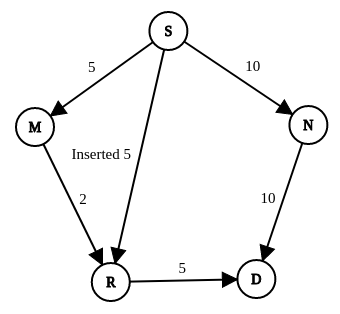
\includegraphics[scale=0.4]{img/insert1.png}
    \caption{Insertion of an edge}
    \label{fig:insert_graph}
\end{figure}
In the graph in Figure~\ref{fig:insert_graph} the Optimal Path before insertion was $S \rightarrow M \rightarrow R \rightarrow D$, when we insert edge $S \rightarrow D$, the cost $f$ of node $R$ changes and Optimal Path changes to $S \rightarrow R \rightarrow D$.


\begin{lemma}\label{lemma:insertion_property1}
Insertion of an edge can not increase the cost of source to destination Optimal Path.
\end{lemma}

\begin{proof}
 Suppose we add and an edge $u \rightarrow v $ with weight $w_{uv}$ where $u \in V$ and $v \in V$. The cost of reaching $v$ from source using edge $u \rightarrow v$ is $g(v)_{new} = g(u) + w_{uv}$. There can be two cases:
\begin{itemize}[label={}]
    \item \textit{Case 1:} If $g(v)_{new} < g(v)$, if optimal path consist of node $v$ then the decrease of cost of $v$ will decrease the cost of Optimal Path, as if there is path from $v$ to destination then source $\rightarrow v \rightarrow$ destination path's cost decreases due to decrease in optimal cost of $v$ thus it becomes the new Optimal Path with lesser cost. if it doesn't then the Optimal Path remains the same.
    
    \item \textit{Case 2:} If $g(v)_{new} \geq g(v)$,  Suppose node $v$ is our destination, from definition Optimal Path is a path with least cost associated with it, so the optimal cost to reach $v$ is $g(v)$, so the addition of this edge has no effect on cost of any node of graph which implies the cost of Optimal Path remains same.
\end{itemize}
In both cases, cost of the Optimal Path doesn't increase, Hence Proved
\end{proof}

\begin{lemma}\label{lemma:insertion_property2}
If we add an edge $u \rightarrow v$ and $f(u) > f(destination)$ then addition of this edge will not affect the Optimal Path.
\end{lemma}
\begin{proof}
 Given  $f(destination) < f(u)$, As weights are positive $w_{uv} > 0$ so cost of any such path from source $\rightarrow u \rightarrow v \rightarrow$ destination will be $g(u) + $ cost of reaching destination from $u$ but as $g(u) > g(destination)$ the cost of such paths will always be larger and hence it can't be the Optimal Path so the addition of such edges doesn't affect the Optimal Path
\end{proof}

\begin{corollary}\label{corollary:insertion_property2}
If If we add an edge $u \rightarrow v$ and $f(u) = \infty$ then addition of this edge will not affect the optimal path.
\end{corollary}
\begin{proof}
 If $f(u) = \infty$ then $f(u) > f(destination)$ so it follows from Lemma \ref{lemma:insertion_property2} that addition of such edges doesn't affect the optimal path.
\end{proof}
We know from Lemma~\ref{lemma:insertion_property1} that insertions can't increase the cost of optimal path but they can decrease the cost, and there can be a new optimal path from the inserted edge. Also if we insert the $u \rightarrow v$ and $g(v)$ changes then all its descendants in the graph whose $g$ are computed based on $v$ are stale values. There can be two approaches to update the cost of graph due to this insertions either \textit{propagate} the new value as insertion took place or compute the new value on demand when necessary i.e \textit{lazy update}. We prefer the first one as it simplifies a lot of computation.

\subsection{Batch Insertion}\label{subsec:batch_ins}
Instead of adding each edge one by one, we process a group of edges inserted at a particular instance of time to utilize the parallelism and computation power of GPU. First, we make an update\_list of vertices from the inserts as if $u \rightarrow v $ is inserted and $f(v)$ decreases then we add $v$ to update\_list. Then until update\_list is empty we expand each child of nodes in update\_list and if the new cost of a child is lesser than the old cost we add the child in update\_list.
\begin{lstlisting}[language=python, caption=Propagation of Insertions,label=algo:prop_ins]
procedure: propagate_insertions( list< pair<u,v> > Inserts, N, E):
    update_list = make_update_list(Inserts);
                          
    while update_list not empty:
        s = size(update_list)
        #array of N elements initialized to 0
        flag = array(N,0)
        #s parallel
        expand(update_list,s,flag)
        #create update list from flag
        update_list = generate_update_list(flag)
        
#GPU kernel
procedure: expand(update_list,s,flag):
    id = global_thread_id;
    node = update_list[id];
    
    for each child ch of node:
        lock(ch)
        if f(ch) > g(node) + weight(node,ch) + h(ch):
            f(ch) = g(node) + weight(node,ch) + h(ch)  
            optimal_parent[ch] = node
            flag[ch] = 1
        unlock(ch)


\end{lstlisting}
At the end of propagation if there is a change in optimal cost then it would also be propagated to the destination node we prove the same below.
\begin{lemma}\label{lemma:insertion_property3}
At the end of propagation, all the nodes $\in V$ have the latest cost  $f$ which is the optimal cost in the new graph including inserts.
\end{lemma}
\begin{proof}
  Suppose we insert edge $u \rightarrow v$. Lets take a node $n \in$ Graph.
\begin{itemize}[label={}]
    \item \textit{Case 1:} If $n \in$ sub-graph($v$), since $v \in$ update list and at each iteration we add nodes which belongs to sub-graph of $v$ and whose $f(n)$ is decreased. According to Lemma \ref{lemma:insertion_property1} Insertion can only decrease the cost, so if $n \in$ update list at some iteration then its $f(n)$ is decreased and that is the new optimal cost $f(n)$, If $n \notin$ update list then $f(n)_{new}$ due to insertion is greater than $f(n)_{old}$ in which case $f(n)_{old}$ is the optimal cost as per the definition of optimal cost.
    \item \textit{Case 2:} If $n \notin$ sub-graph($v$) which implies that there can be no change in the optimal\_path from source to $n$ (as there is no structural change in this part of graph), thus it's cost remains unchanged and which is the optimal cost of node $n$ in new graph.
\end{itemize}
\end{proof}
\begin{lemma}\label{lemma:insertion_property4}
At the end of propagation $f(destination)$ is the optimal cost of reaching destination from $source$ in the new graph G(V, E+Inserts ).
\end{lemma}
\begin{proof}
  Follows from Lemma~\ref{lemma:insertion_property3}, $destination \in V$, so at the end of propagation $f(destination)$ is the optimal cost i.e optimal cost of reaching $destination$ from $source$ in new graph including inserts i.e G(V, E+Inserts )
\end{proof}

\section{Decremental Processing}\label{sec:decremental}
In Decremental setting there are only removal of edges $u \rightarrow v$ where $u \in V$ and $v \in V$. Addition of edges can only reduce the Optimal Cost (Lemma~\ref{lemma:insertion_property1}), whereas deletion of edges can increase the Optimal Cost (Lemma~\ref{lemma:deletion_prop1}) and can also make the graph disconnected, which poses a new problem as the new optimal path may contain many nodes which are not even explored yet. Further, if multiple deletions are happening at the same time one can read stale values for the path which doesn't even exist in the new graph. This extra set of problems requires some extra computation which makes deletion computationally costlier than the insertions.
% \todo{highlight the challenge due to edge deletion -- which is not present in incremental setting.}
\begin{figure}[H]
    \centering
    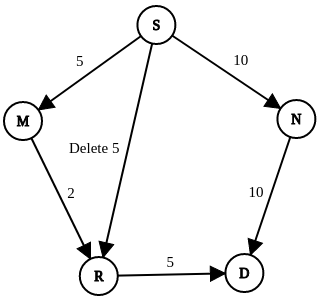
\includegraphics[scale=0.4]{img/Delete2.png}
    \caption{Deletion of an edge}
    \label{fig:delete_sample}
\end{figure}
In the example graph in Figure~\ref{fig:delete_sample} the Optimal Path before deletion was $S \rightarrow R \rightarrow D$, when we delete the edge $S \rightarrow R$, the Optimal Path changes to $S \rightarrow M \rightarrow R \rightarrow D$.\\
Below we prove some important properties that holds when we remove edges from graph. The following properties holds when we have the Optimal Path for the graph before deletions.
\begin{lemma}\label{lemma:deletion_prop1}
Deletion of edge $ u \rightarrow v$ where $u \in V$ and $v \in V$ can not decrease $f(v)$.
\end{lemma}
\begin{proof}
  Let edge $ u \rightarrow v$ gets deleted from graph then,
\begin{itemize}[label={}]
    \item \textit{Case 1:} If $u =$ optimal\_parent($v$) then, source $\rightarrow u \rightarrow v$ was the optimal path of reaching $v$ from source, So after deletion, $f(v)_{new} = g(s) + w_{sv} + h(v)$ where $s$ is parent of $v$ with least $g$, In A* we chose the path with least $f$ as we chose $u$ before $s$ implies $f(v)_{new} \geq f(v)_{old}$.
    \item \textit{Case 2:} If $u$ is  not the optimal\_parent($v$), then let $s$ be the optimal\_parent($v$), deletion of edge $u \rightarrow v$ doesn't affect the $f(v)$ as the least cost of reaching $v$ is from $s$.
\end{itemize}
From above we can say that deletion of edge $u \rightarrow v$ can only increase $f(v)$. Hence Proved.
\end{proof}
\begin{lemma}\label{lemma:deletion_prop2}
If edge($u,v$) $\notin$ Optimal Path, then deletion of such edges doesn't affect the Optimal Path.
\end{lemma}
\begin{proof}
  Suppose we delete edge($u,v$) $\notin$ Optimal Path then, as from Lemma~\ref{lemma:deletion_prop1} deletion of such edges can only increase $f(v)$ so if there is a path from source $\rightarrow v \rightarrow$ destination then it's cost will be increased, as Optimal Path is least-cost path such paths cannot be an Optimal Path, Hence deletion of such edges doesn't affect the Optimal Path.
\end{proof}

\begin{lemma}\label{lemma:deletion_prop3}
If edge(u,v) is deleted and optimal\_parent(v)$\neq$u, then deletion of such edges doesn't affect the Optimal Path.
\end{lemma}
\begin{proof}
  If $u$ is  not the optimal\_parent($v$), then let $s =$ optimal\_parent($v$), deletion of edge $u \rightarrow v$ doesn't affect the $f(v)$ as the least cost of reaching $v$ is from $s$, as there is no change in cost of any nodes so Optimal Path remains same.
\end{proof}

\subsection{Batch Deletion}\label{subsec:batch_del}
Instead of deleting edges one by one we process deletion in batches, where a batch contains all the deleted edges before a query. From Lemma~\ref{lemma:deletion_prop1} we know that deletion of edges can increase the optimal cost, to compute the new optimal cost, we first propagate the change in cost due to deletion of edges to all affected nodes and then we perform a check that we are not violating the Lemma~\ref{lemma:Astar property} after propagation, which is an essential property to always hold so that later we can process the next incoming updates, if it violates Lemma~\ref{lemma:Astar property} then we start A* from where we left before i.e using the open\_list we have computed before. In the end, we will have the new Optimal Path with the optimal cost for new graph encompassing all the deletions.\\
\\
\textit{Propagation for Deletion:}
\begin{enumerate}
    \item For each deleted edge $u \rightarrow v$, if $f(v) \neq \infty$ and optimal\_parent($v$)$=u$ then for such edges we compute the cost of reaching $v$ from its parent's and chose the least one as optimal\_parent($v$) and update $f(v)$, if $v$ doesn't have any parent then $f(v)=\infty$, and we add $v$ to update\_list.
    
    \item For each child of nodes in update\_list, we compute the cost $f$ of child with respect to node and If new cost $f$ is more than $f(child)$ and optimal\_parent(child)  is node then, we compute the cost of reaching child from all of its parents and update $f$ to the least cost of the parents and set that parent as optimal\_parent. And we add the child to the next update\_list.
    
    \item We repeat steps 1 and 2 until update\_list is empty.
\end{enumerate}
Optimal Cost is least cost of reaching the node but we increase the cost of the child at step 2 in the above procedure, why we do that is because from Lemma~\ref{lemma:deletion_prop1} we know that $f$ might increase due to deletion of edges and we need to propagate the updated higher cost. Also since there is no special ordering of nodes to execute the propagation it may happen that while we are propagating for a node its sub-graph might already have been updated so to make sure we have latest cost value among those, we choose the least cost parent and then propagate that cost downwards if applicable.
\begin{figure}[H]
    \centering
    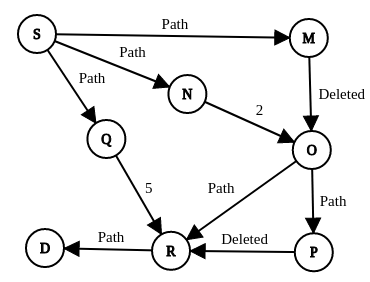
\includegraphics[scale=0.4]{img/Delete1.png}
    \caption{Batched deletion of multiple edges}
    \label{fig:delete_multiple}
\end{figure}

In the example graph in Figure~\ref{fig:delete_multiple}, the Optimal Path before deletion is $S \rightarrow M \rightarrow O \rightarrow P \rightarrow R \rightarrow D $.
The edges $ M \rightarrow O$ and $P \rightarrow R$ are deleted from graph. So $R,O \in $ update\_list, While propagating for $O$ we might find $R$ again from path $O \rightarrow R$ but $R$ has already updated, if in that update $R$ has chosen path $S \rightarrow M \rightarrow O \rightarrow R$ as its Optimal Path then we have stale value for $f(R)$ as $M \rightarrow O$ is deleted but since $R$'s update happened first it read the stale value before propagation. In such cases, we need to find the parent with the least cost thus we compute the cost of reaching node from all its parents and choose the parent with the least cost as optimal\_parent.

\subsection{Deletion and Cycles}\label{subsec:del_cycle}
We propagate the deletions so that each node whose cost is already computed will have the latest value. There is a special case of deletions with a cycle where even after propagation we can get stale value if we don't perform certain checks while propagating the latest value to nodes. as given in the example below:
\begin{figure}[H]
    \centering
    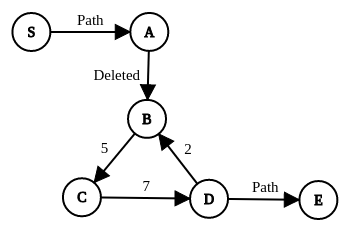
\includegraphics[scale=0.45]{img/cycle.png}
    \caption{Deletion in Cyclic Graphs }
    \label{fig:delete_cycle}
\end{figure}
In the example graph in Figure~\ref{fig:delete_cycle} the Optimal Path is from $S \rightarrow ABCD \rightarrow E$, where $S$ is source and $E$ is destination. When we remove the edge $A \rightarrow B$, and recompute the $f(B)$, there exist only one parent $D$ so the $f(B)_{new}$ is computed by $f(B)_{new} = g(D) + 2 + h(B)$, which is old value of $g(D)$, as we remove $A \rightarrow B$, there is no path from $S \rightarrow D$ so $g(D)_{new}$ is $\infty$, but we never arrive at that proposition because in propagation of deletion we will propagate from $B$  and $f(D)$ will be updated based on stale value of $f(B)$ and thus we have wrong cost value after deletion of such edges. The main reason this happens is due to the fact that cost $f(D)$ is computed wrt $B$ as $B \in OptimalPath(S,D)$. To avoid such cases, while choosing the optimal\_parent we have to eliminate the parents whose Optimal\_ancestor is current node.\\
\begin{lstlisting}[language=python, caption=Check Cycles]
procedure: check_cycle(node,parent):
    current_node = node
    while there exists optimal_parent(current_node):
        if current_node == parent:
            return true
        current_node = optimal_parent(current_node)
    
    return false
\end{lstlisting}

\subsection{Parallel Deletion and Cycle}\label{subsec:parallel_cycle}
When there are multiple deletions happening at the same time, there can be a cycle of optimal\_parent, and thus when we do the above check, we get into an infinite loop also we defined optimal\_parent as a non-cyclic path to start node. To eliminate such a cycle when we process deletion we have to do additional processing of removing such cycles.
\begin{figure}[H]
    \centering
    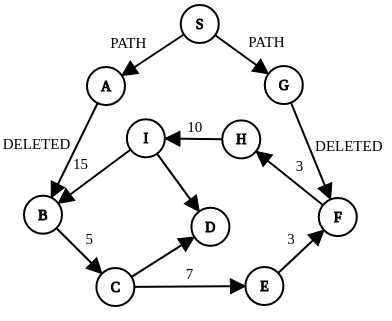
\includegraphics[scale=0.45]{img/Delete_cycle.png}
    \caption{Parallel Deletion in Cyclic Graphs}
    \label{fig:delete_parallel_cycle}
\end{figure}

In the example graph in Figure~\ref{fig:delete_parallel_cycle}, the Optimal Path from $S\rightarrow D$ is $SABCD$,when we delete edges $A \rightarrow B$ and $G \rightarrow F$,for node $B$ the new parent is $I$ as $B \notin optimal\_parents(I)$, also the new parent of $F$ becomes $E$ as $E \notin optimal\_parents(F)$ this is because we are checking for optimal\_parent for both nodes in parallel thus the check happens at the same time and both reads the optimal\_parent values before it gets changed by either one of them. Thus forming a cycle of optimal\_parents which violates our definition of optima\_parent, to solve this we perform additional cycle check after each iteration of propagation for deletion and if such cycle found we remove them.\\
Now the question arises to remove which newly formed edge of the cycle i.e remove $I= $optimal\_parent($B$) or remove $E=$ optimal\_parent($F$). which one belongs to the optimal path? the answer is we can just remove any of cycle edges and our propagation algorithm will take care of which edge actually belong to the cycle.\\

%explain HOW

The propagation for deletion handling all the above cases is given below:
\begin{lstlisting}[language=python, caption=Propagation of Deletions]
procedure: propagate_deletions( list< pair<u,v> > Deletions, E, N):
     update_list = make_update_list(Deletions);
     check_optimal_parent_cycle(update_list);
     
     while update_list not empty:
        s = size(update_list)
        #array of N elements initialized to 0
        flag = array(N,0)
        #s parallel
        expand(update_list,s,flag)
        
        #create update list from flag
        update_list = generate_update_list(flag)
        
        #remove optimal_parent cycle 
        check_optimal_parent_cycle(update_list);

#GPU kernel
procedure: expand(update_list,s,flag):
    id = global_thread_id;
    node = update_list[id];
    
    for each child ch of node:
        lock(ch)
        
        if f(ch) > g(node) + weight(node,ch) + h(ch):
            f(ch) = g(node) + weight(node,ch) + h(ch)  
            optimal_parent[ch] = node
            flag[ch] = 1
        
        else if f(ch) < g(node) + weight(node,ch) + h(ch) and optimal_parent[ch] == node:
            for all parents p of ch:
            
                if check_cycle(ch,p) == true:
                    continue
            
                if f(ch) > g(p) + weight(p,ch) + h(ch):
                    f(ch) = g(p) + weight(p,ch) + h(ch)
                    optimal_parent[ch] = p
            
            flag[ch] = 1
        
        unlock(ch)
        
\end{lstlisting}

\begin{lemma}\label{lemma:deletion_prop4}
At the end of propagation for deletion all node  $ n \in V$  such that $f(n)_{new} \neq \infty $ has the latest $f(n)$ which is optimal cost in new graph including deletions.
\end{lemma}
\begin{proof} Suppose we delete edge $u \rightarrow v$. Let node $n \in V$:\\
\textit{Case 1:} If $n \in$ sub-graph($v$) then there can be two sub-cases: \begin{enumerate}
\item If $v \in$ Optimal\_Path($n$) which implies $f(n) \neq \infty$, when we add $v$ in update\_list we compute the least cost of reaching $v$ from all of its remaining parent we also make sure that the parent we chose is such that its cost in not computed wrt $v$ which implies its the optimal\_cost of reaching $v$. Since $v \in$ Optimal\_Path($n$) , $\exists$ parent $p$ of $n$ such that $p \in$ Optimal\_Path($n$) and $p \in$ sub-graph($v$), which implies $p \in$ update\_list at some iteration of propagation, when $p$ tries to update $n$, $n$ will chose the best available parent thus cost of $f(n)$ is optimal\_cost of reaching $n$ in new graph.
\item If $v \notin$ Optimal\_Path($n$),then $\exists$ optimal\_parent $p$ of n such that $v \notin $ Optimal\_Path($p$), thus $n \notin$ update\_list at any iteration of propagation so $f(n)$ remains same which is the optimal\_cost from Lemma~\ref{lemma:deletion_prop2}. 
\end{enumerate}
\textit{Case 2:} If $n \notin$ sub-graph($v$) then $v \notin$ Optimal\_Path($n$) also $v \notin$ update\_list at any iteration of propagation so $f(n)$ remains same which is the optimal\_cost from Lemma \ref{lemma:deletion_prop2}
\end{proof}

\begin{lemma}\label{lemma:deletion_prop5}
At the end of propagation $f(destination)$ might not be the optimal cost of reaching destination from source in new graph.
\end{lemma}
\begin{proof}
\begin{figure}[H]
    \centering
    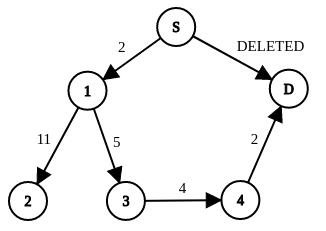
\includegraphics[scale=0.4]{img/del_prop.png}
    \caption{}
    \label{fig:deletion_proof}
\end{figure}
To prove, It is sufficient to give an example where $f(destination)$ is not the optimal cost after propagation for deletion.\\
In the graph in Figure~\ref{fig:deletion_proof} at the end of A* we will have:\\
open\_list : \{2,3\}\\
closed\_list : \{S,1,D\}\\
Thus node 4 is not visited thus having $f(4)=\infty$, after propagation for deletion as D has only one parent 4 its cost is computed wrt 4 so $f(D)=\infty$, but int the new graph the optimal cost is $f(D)=13$ with Optimal\_Path $S\rightarrow 1\rightarrow 3 \rightarrow 4 \rightarrow D$.\\
Thus in above graph $f(D)$ after the propagation of deletion is not the optimal cost in new graph.  
\end{proof}

\begin{lemma}\label{lemma:deletion_prop6}
After propagation of deletions if $f(destination) < f(n)$ $ \forall$ $n \in $open\_list then $f(destination)$ is the optimal cost of reaching destination from source.
\end{lemma}
\begin{proof}
After propagation of deletion $\forall$ node $n \in $ open\_list either $f(n)_{new}$ is the optimal\_cost or $f(n)_{new} = \infty$, from Lemma~\ref{lemma:deletion_prop4}. Also given $f(destination) < f(n)$ $ \forall$ $n \in $open\_list, As weights are non-negative so for all descendants of $n$ $f($ descendants $) > f(n)$. So reaching $destination$ from any node in update\_list will have larger cost than current value, thus $f(destination)$ is the optimal cost of reaching destination from source.
\end{proof}

From Lemma~\ref{lemma:deletion_prop5} we know that after propagation for deletion $f(destination)$ is not the optimal cost, also from Lemma~\ref{lemma:deletion_prop6} we know that if $f(destination) < f(n)$ $ \forall$ $n \in $ open\_list then $f(destination)$ is the optimal cost, to satisfy the this condition we need to perform A* after propagation for deletion as after A* $f(destination) < f(n)$ $ \forall$ $n \in $open\_list and thus $f(destination)$ is the optimal cost.
\begin{lstlisting}[language=python, caption= Procedure for Deletions]
procedure: Deletions(list< pair<u,v> > deleted_edges,N,E)
    propagate_deletions(deleted_edges,N,E);
    # A* from old saved state
    GA*(open_list,closed_list,source,destination,K)

\end{lstlisting}
%explanation about why we need A* after this.
\section{Fully Dynamic}\label{sec:fully_dynamic}
Real-world graphs are dynamic and edges are changing continuously so there are the insertions of edges and deletion of edges at the same instance in such cases if a query is raised to find the optimal path from source to the destination we can retrieve the optimal path without re-executing A* from start again.

\subsection{Separate Propagation}\label{subsec:sep_propagation}
As we have already discussed how to find the optimal path when edges are either added only or deleted only we can infer the dynamic change in edges at a single instance as addition happening first then deletion or vice versa. So we process addition first as insertion only then we process deletion as deletion only. It may happen that some nodes will get updated multiple times in two different propagation. But as insertion and deletion require a different set of instruction it is a good choice to separate the propagation.
\begin{lstlisting}[language=python, caption=Separate Propagation]
procedure: separate_propagation(list< pair<u,v> > inserted_edges,list< pair<u,v> > deleted_edges,N,E)
    propagate_insertions(inserted_edges,N,E)
    propagate_deletions(deleted_edges,N,E)
    # A* from old saved state
    GA*(open_list,closed_list,source,destination,K)
\end{lstlisting}

\begin{lemma}\label{lemma:sep_propagation_correctness}
After separate propagation $f(destination)$ is the optimal cost of reaching destination from source in new graph including insertion and deletions.
\end{lemma}
\begin{proof}
In separate propagation first we propagate for insertions and as from Lemma~\ref{lemma:insertion_property4} at end of it we have $f(destination)$ as the optimal cost in new graph which includes all inserted edges.
In the new graph, we propagate for deletions and then perform GA* so from Lemma~\ref{lemma:deletion_prop6} we have $f(destination)$ as the optimal cost in the graph which includes both insertion and deletion. Thus $f(destination)$ is the optimal cost of reaching the destination from the source in the new graph including insertion and deletions.
\end{proof}

\subsection{Simultaneous Propagation}\label{subsec:sim_propagation}
We have designed the propagation of Insertion(section ~\ref{subsec:batch_ins}) and propagation of deletions (section \ref{subsec:batch_del}) such some parts of them can be overlapped and we can process both insertion and deletion at the same time by considering them as an update. But since both propagations are happening at the same time there are few additional cases we need to take care of thus adding some more checks as given below.

\subsubsection{Insert-Delete Cycle}\label{subsec:ins_del_cycle}
Since we have insertions and deletions propagating at the same time, If we don't perform enough checks we can get into cycles for certain cases. 
\begin{figure}[H]
    \centering
    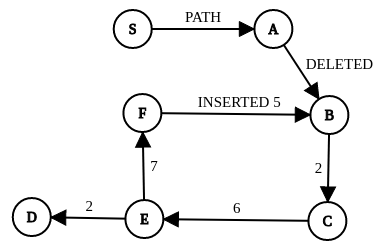
\includegraphics[scale=0.45]{img/ins_del_cycle.png}
    \caption{Cyclic graph with parallel insertion and deletion}
    \label{fig:insert_delete_cycle}
\end{figure}
In the graph in Figure~\ref{fig:insert_delete_cycle} we remove $A \rightarrow B$ and insert $F \rightarrow B$, Due to deletion $f(B) = \infty$, when we propagate for edge $F \rightarrow B$,the cost of reaching $B$ from $F$ via newly added edge is less than infinity thus, we compute the new cost and make optimal\_parent($B$) = $F$,But when we try to to retrace the path from $F$ to $S$ we get $F\rightarrow E\rightarrow C\rightarrow B\rightarrow F...$ thus we have a optimal\_parent cycle. It is because the cost of $F$ itself is a stale value due to the fact that its cost is computed wrt to $B$ and deleted edge $A \rightarrow B$. To remove such cases we have to extensively check for insertion of edges $u \rightarrow v$, if $v \in $optimal\_parents($u$) for all insertions.

\subsubsection{Propagation Cycle}\label{subsec:propagation_cycle}
Since Insertions and Deletions are propagating at the same if there is a cycle and each reaches the cycle at different iterations, It might happen due to the structure of the graph that they propagate indefinitely on such cycles if the check mentioned in the above section is not implemented for each insertion.
\begin{figure}[H]
    \centering
    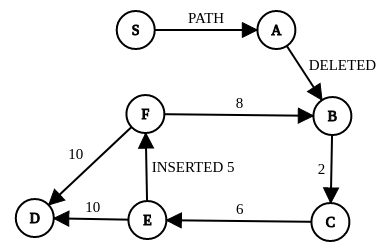
\includegraphics[scale=0.45]{img/prop_cycle.png}
    \caption{Infinite propagation due to formation of cycles}
    \label{fig:propogation_cycle}
\end{figure}

In the graph in Figure~\ref{fig:propogation_cycle} $A \rightarrow B$ is deleted and $E \rightarrow F$ is added. Due to deletion cost of $B = \infty$  and due to insertion cost of $F$ is changed in next iteration cost of $C = \infty$ as there is no path from $S \rightarrow C$ in new graph, also due to edge $f \rightarrow B$ the cost of $B$ is changed as the new cost is less than $\infty$. In the next iteration cost of $E = \infty$ and cost of $C$ is changed, Similarly in the next iteration cost of $F = \infty$, and cost of $E$ is changed, and similarly the propagation goes on the loop indefinitely. The problem here is we computed the cost of $B$ from $F$ when $F$ has the stale value and its cost is computed wrt $B$ itself. This can be removed by doing the check mentioned in the above section~\ref{subsec:del_cycle}.

\begin{lstlisting}[language=python, caption=Propagation of Updates]
procedure: propagate_updates( list< pair<u,v> > Deletions,list< pair<u,v> > Inserts, E, N):
     update_list = make_update_list_insertion(Inserts);
     update_list = append( update_list, make_update_list_deletion(Deletions) )
     
     while update_list not empty:
        s = size(update_list)
        #array of N elements initialized to 0
        flag = array(N,0)
        #s parallel
        expand(update_list,s,flag)
        #create update list from flag
        update_list = generate_update_list(flag)

#GPU kernel
procedure: expand(update_list,s,flag):
    id = global_thread_id;
    node = update_list[id];
    
    for each child ch of node:
        lock(ch)
        
        if f(ch) > g(node) + weight(node,ch) + h(ch):
            f(ch) = g(node) + weight(node,ch) + h(ch)  
            optimal_parent[ch] = node
            flag[ch] = 1
        
        elif f(ch) < g(node) + weight(node,ch) + h(ch) and optimal_parent[ch] == node:
            for all parents p of ch:
             
                if check_cycle(ch,p) == true:
                    continue
             
                if f(ch) > g(p) + weight(p,ch) + h(ch):
                    f(ch) = g(p) + weight(p,ch) + h(ch)
                    optimal_parent[ch] = p
            
            flag[ch] = 1
        
        unlock(ch)
\end{lstlisting}


\section{Experimental Results}\label{sec:experiments}
%results
%setup and GPU specs
In this section, we have compared the performance of our algorithm with multiple GPU A* algorithms. We also discuss how various parameters affect the performance of our algorithm(DA*). The GPU we used the experiments is a Tesla K40c which has 15 SM each having 192 cores(total 2880 cores), it has 12 GB of Global Memory and has a clock rate of 740 MHz.

The performance of GPU A*(GA*)\cite{GA*} is dictated by the expansion of nodes simultaneously which is restricted by how many parallel priority queues are created. As we increase the number of priority queues the execution time decreases because we process a large number of nodes in parallel. The trend follows as shown in Figure~\ref{fig:runtime_K}.

\begin{figure}[H]
    \centering
    \begin{subfigure}[b]{0.50\textwidth}
        \centering
        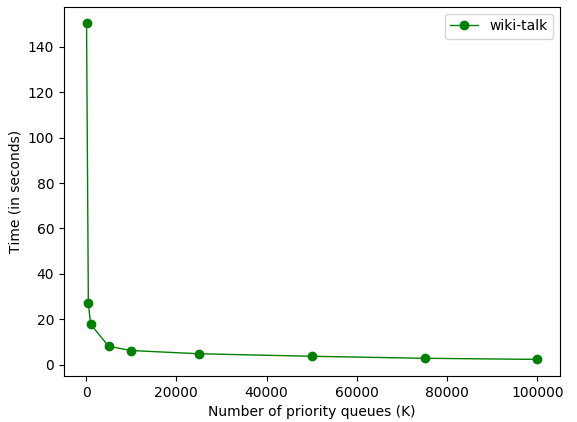
\includegraphics[width=\textwidth]{img/RvK.png}
        \caption{Execution Time vs Number of Parallel Priority Queues}
        \label{fig:runtime_K}
    \end{subfigure}
    \hfill
    \begin{subfigure}[b]{0.47\textwidth}
        \centering
        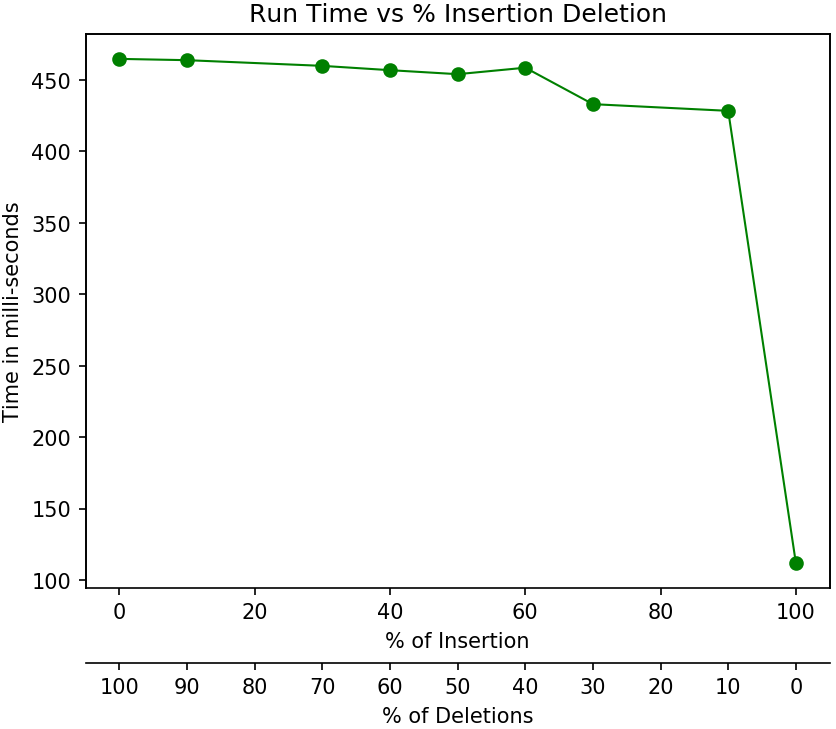
\includegraphics[width=\textwidth]{img/IDvK.png}
        \caption{Execution Time vs Edge density}
        \label{fig:edge_dens}
    \end{subfigure}
    \caption{}
\end{figure}

When the graph is only subjected to the insertion of edges, the amount of processing required to find the new optimal path is based on how many nodes are being affected ( cost change ) due to the insertions, which generally increases as we increase the number of edges being inserted. Figure~\ref{fig:insert_trend} shows the increase in execution time, we can also infer that the increase is linear for certain part of in each sub-figure. In Figure~\ref{fig:insert_trend_3} there is a dip then rise, it is because initially the destination node was unreachable so it has to process all nodes and as we keep inserting edges the source-destination path is created and it then became shorter as more edges got inserted in graph, after a while due to increase in number of edges the size of the graph grew and also the number of nodes which are updated simultaneously grew so contention for lock increases thus increasing the execution time.
\begin{figure}[H]
    \centering
    \begin{subfigure}[b]{0.42\textwidth}
         \centering
         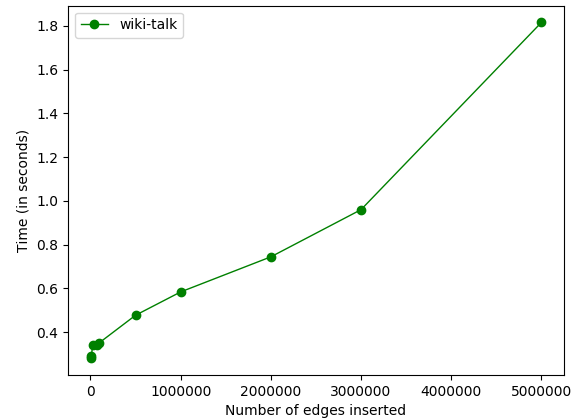
\includegraphics[width=\textwidth]{img/ins/i0.png}
         \caption{}
         \label{fig:insert_trend_1}
    \end{subfigure}
    \hfill
    \begin{subfigure}[b]{0.45\textwidth}
         \centering
         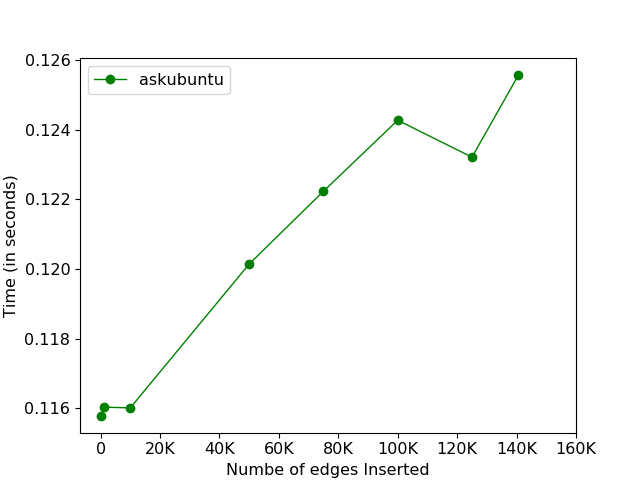
\includegraphics[width=\textwidth]{img/ins/i1.png}
         \caption{}
         \label{fig:insert_trend_2}
    \end{subfigure}
    \hfill
    \begin{subfigure}[b]{0.45\textwidth}
         \centering
         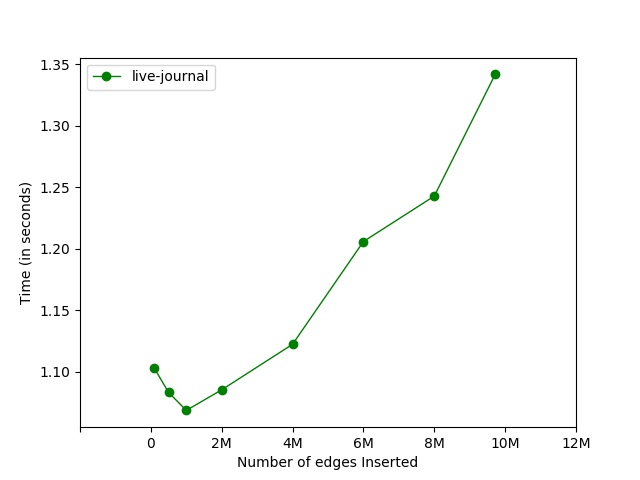
\includegraphics[width=\textwidth]{img/ins/i2.png}
         \caption{}
         \label{fig:insert_trend_3}
    \end{subfigure}
    \hfill
    \begin{subfigure}[b]{0.45\textwidth}
         \centering
         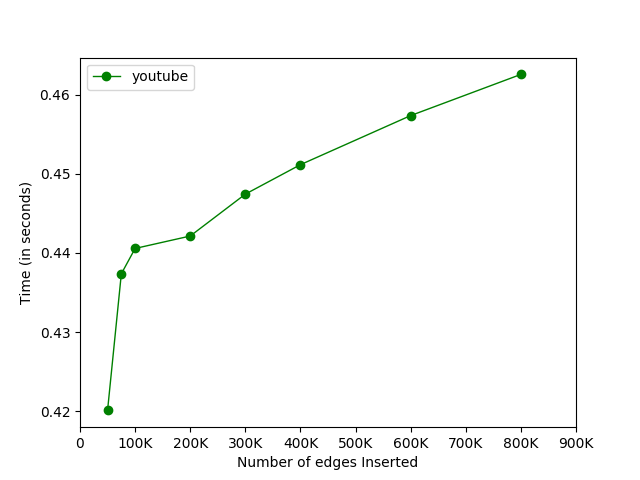
\includegraphics[width=\textwidth]{img/ins/i3.png}
         \caption{}
         \label{fig:insert_trend_4}
    \end{subfigure}
    
    \caption{Execution time when graph is only subjected to Insertions}% \todo{increase font size}}
    \label{fig:insert_trend}
\end{figure}

Similarly for deletion as deletion size increases we need to process more nodes,and contention at lock also increases thus increases the execution time, as shown in Figure~\ref{fig:deletion_trend}. We also observe that there are certain points where the execution time increase drastically in each Figure~\ref{fig:deletion_trend_1},~\ref{fig:deletion_trend_2},~\ref{fig:deletion_trend_3},~\ref{fig:deletion_trend_4} It might be due to the sudden increase in number of edges i.e $(u \rightarrow v)$ deleted which are part of optimal path to the node $v$, which increase the amount of processing required.
\begin{figure}[H]
    \centering
    \begin{subfigure}[b]{0.48\textwidth}
         \centering
         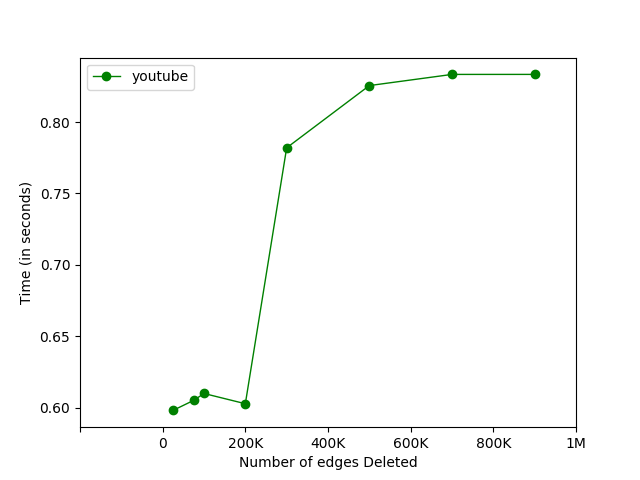
\includegraphics[width=\textwidth]{img/del/d1.png}
         \caption{}
         \label{fig:deletion_trend_1}
    \end{subfigure}
    \hfill
    \begin{subfigure}[b]{0.48\textwidth}
         \centering
         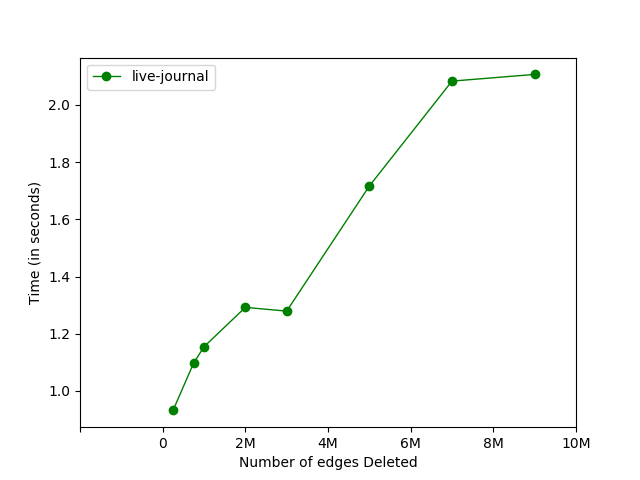
\includegraphics[width=\textwidth]{img/del/d2.png}
         \caption{}
         \label{fig:deletion_trend_2}
    \end{subfigure}
    \hfill
    \begin{subfigure}[b]{0.48\textwidth}
         \centering
         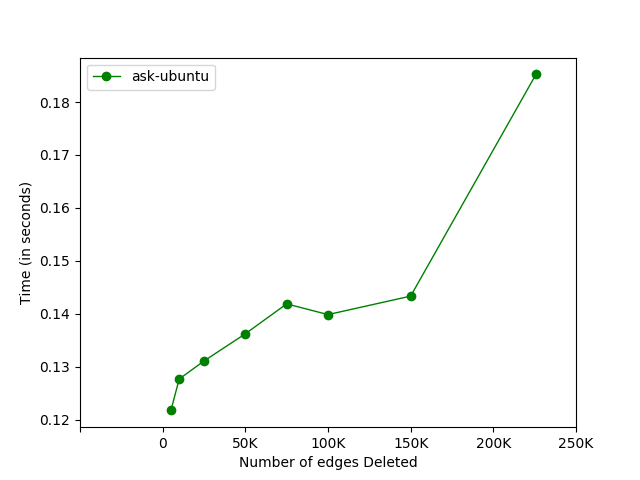
\includegraphics[width=\textwidth]{img/del/d3.png}
         \caption{}
         \label{fig:deletion_trend_3}
    \end{subfigure}
    \hfill
    \begin{subfigure}[b]{0.48\textwidth}
         \centering
         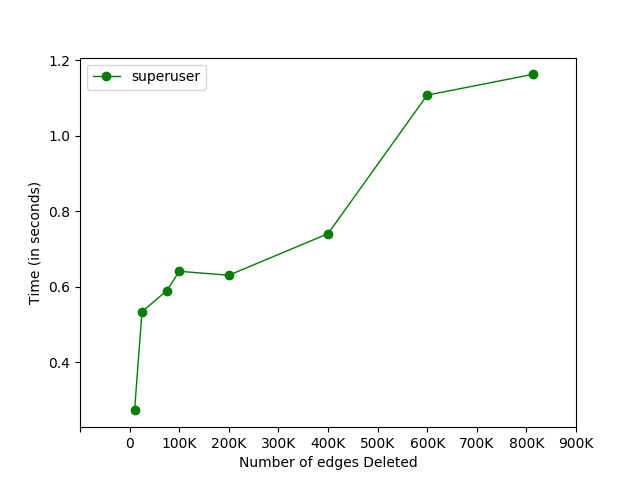
\includegraphics[width=\textwidth]{img/del/d4.png}
         \caption{}
         \label{fig:deletion_trend_4}
    \end{subfigure}
    \caption{Execution time when graph is only subjected to Deletions|}% \todo{increase font size in plots along x and y axes.}}
    \label{fig:deletion_trend}
\end{figure}

In a dynamic setting when we process both insertion and deletion at the same time. With an increase in the number of Updates, the execution time increases as in Figure~\ref{fig:dynamic_trend}. We can also observe that the sub-figures looks more similar to Figure~\ref{fig:deletion_trend} that is because propagation for deletion takes more computation power than for insertion.
\begin{figure}[H]
    \centering
    \begin{subfigure}[b]{0.45\textwidth}
         \centering
         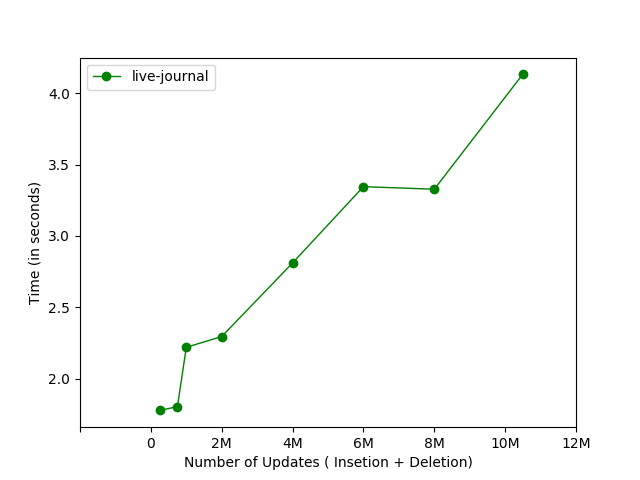
\includegraphics[width=\textwidth]{img/dyn/u1.png}
         \caption{}
         \label{fig:dynamic_trend_1}
    \end{subfigure}
    \hfill
    \begin{subfigure}[b]{0.45\textwidth}
         \centering
         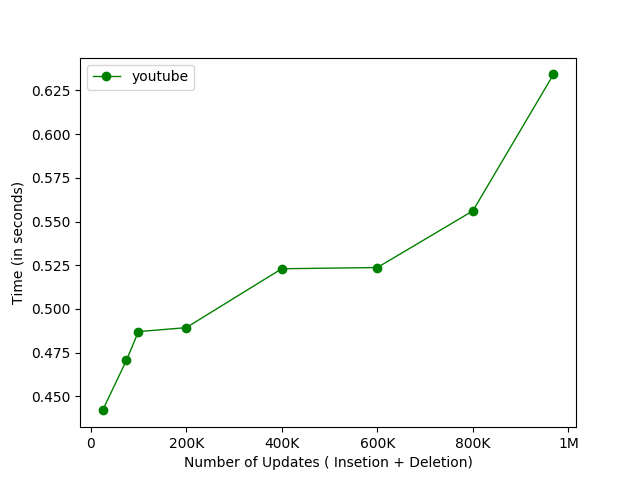
\includegraphics[width=\textwidth]{img/dyn/u2.png}
         \caption{}
         \label{fig:dynamic_trend_2}
    \end{subfigure}
    \hfill
    \begin{subfigure}[b]{0.45\textwidth}
         \centering
         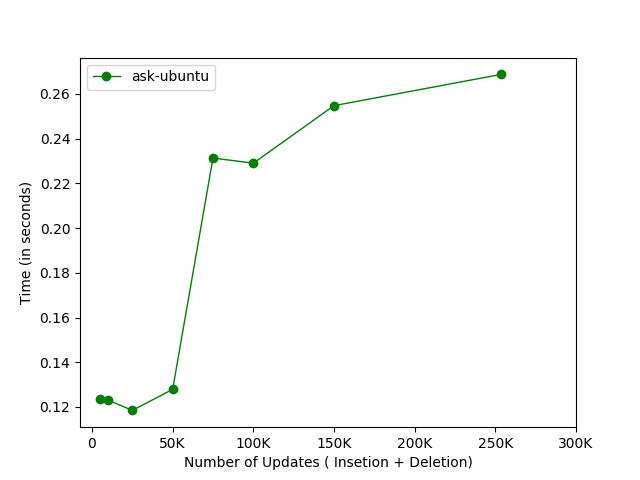
\includegraphics[width=\textwidth]{img/dyn/u3.png}
         \caption{}
         \label{fig:dynamic_trend_3}
    \end{subfigure}
    \hfill
    \begin{subfigure}[b]{0.45\textwidth}
         \centering
         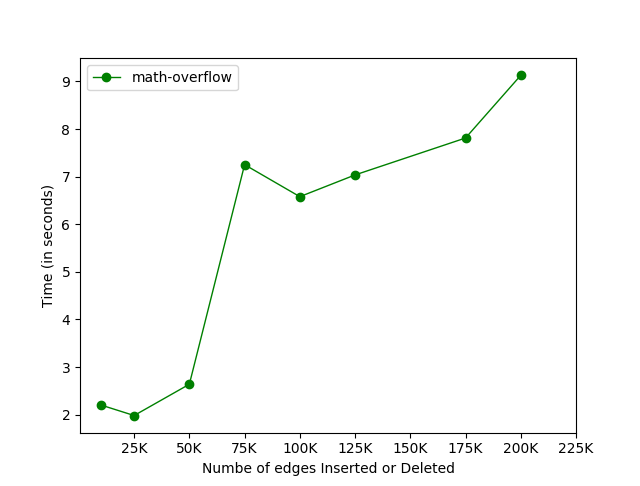
\includegraphics[width=\textwidth]{img/dyn/u4.png}
         \caption{}
         \label{fig:dynamic_trend_4}
    \end{subfigure}
    \caption{Execution time vs Number of Updates}
    \label{fig:dynamic_trend}
\end{figure}
The amount of execution time needed to process deletion is much larger than inserts. As shown in Figure~\ref{fig:runtime_ins_del} where the total number of updates is kept constant but the amount of updates which are insertion or deletion is changed we observe that there is a drastic drop in execution time as the percentage of deletion becomes 0. It shows that even for a small amount of deletion the execution time is high compared to insertions. It is because we are performing multiple checks for the cycle when we process deletion which takes a major amount of execution time, while in insertion there is no need to check for the cycle when we are doing separate propagation. In Figure~\ref{fig:DA_version} we compare the two variants of DA*, simultaneous propagation and separate propagation, separate propagation outperforms simultaneous propagation as the later require more computation for the additional checks as discussed in section~\ref{subsec:ins_del_cycle} and section~\ref{subsec:propagation_cycle}.
\begin{figure}[H]
    \centering
    \begin{subfigure}[b]{0.44\textwidth}
        \centering
        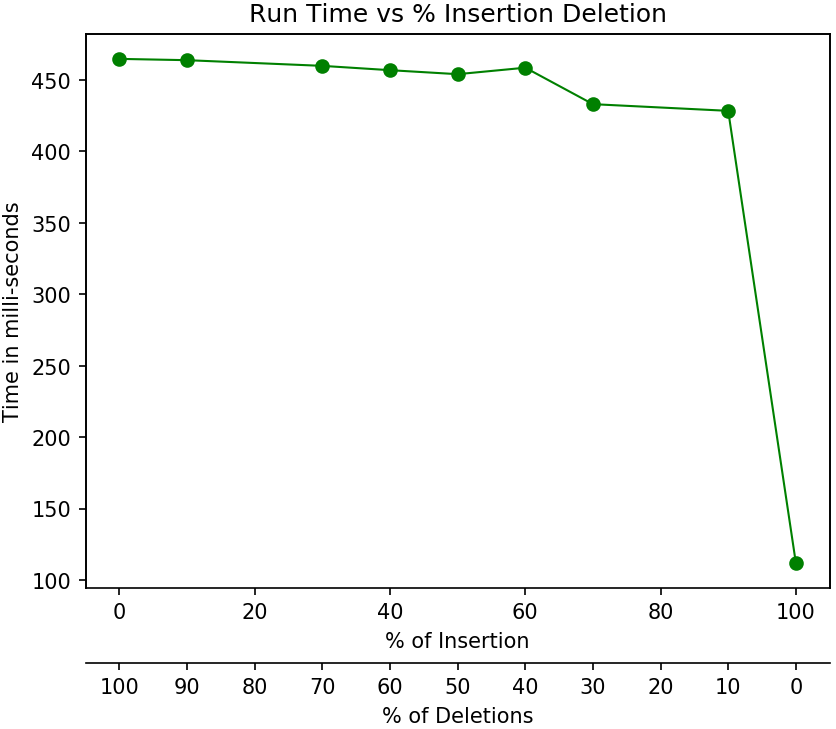
\includegraphics[width=\textwidth]{img/IDvK.png}
        \caption{Run Time vs \% Insert/Delete}
        \label{fig:runtime_ins_del}
    \end{subfigure}
     \hfill
    \begin{subfigure}[b]{0.50\textwidth}
        \centering
        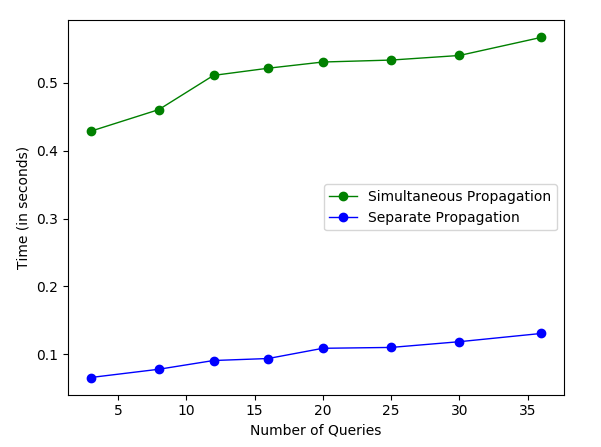
\includegraphics[width=\textwidth]{img/propagation_method.png}
        \caption{Different version of DA* propagation}
        \label{fig:DA_version}
    \end{subfigure}
   \caption{}
    
\end{figure}

Here we compare the performance of our algorithm than by doing GPU A* repeatedly. The below Figure~\ref{fig:query_trend} shows how execution time varies when we increase the number of queries ( finding the path from source to destination after some update ) increases. Performing  GA* after each set of updates is almost linear but propagating the updates as described in the above sections takes considerably less amount of execution time. The speed-up we can get is proportional to the number of queries we preform, as the number of queries increases we get the better and better speed up. In the Figure~\ref{fig:query_trend_ins} updates only consist of \textit{inserts} while the Figure~\ref{fig:query_trend_dyn} consisting of both insertion and deletion. In Figure~\ref{fig:query_trend_dyn} we can infer that when the number of queries is 1 multiple GA* perform better than Dynamic A* but as we increase the number of queries Dynamic A* perform better than multiple GA*. The speedup we get by applying our algorithm is proportional to the number of queries ( updates ) graph is subjected to, we also have seen an increase in speedup as the size (nodes, edges) of graph increases. To test the capability of our algorithm we used real-world temporal graphs and networks taken from SNAP~\cite{SNAP} results shown in table~\ref{tab:comparison}. We got 37x speedup for 100 queries.
\begin{figure}[H]
    \centering
    \begin{subfigure}[b]{0.47\textwidth}
         \centering
         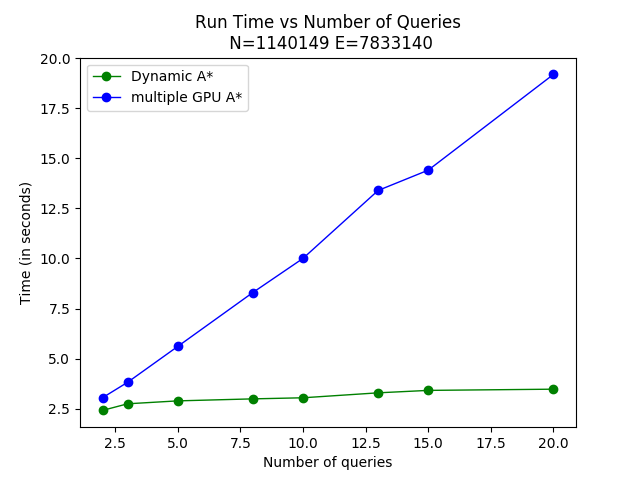
\includegraphics[width=\textwidth]{img/TvQ_wikitalk.png}
         \caption{Only Insertions}
         \label{fig:query_trend_ins}
    \end{subfigure}
    \hfill
    \begin{subfigure}[b]{0.47\textwidth}
        \centering
         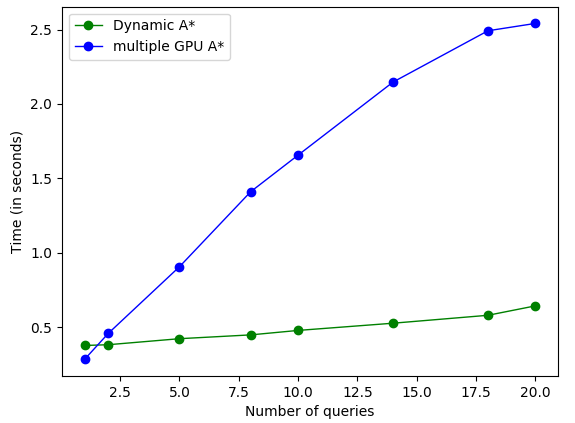
\includegraphics[width=\textwidth]{img/QvT_dyn.png}
         \caption{Both Insertions and Deletions}
         \label{fig:query_trend_dyn}
    \end{subfigure}
    \caption{Execution Time vs Number of Queries}
    \label{fig:query_trend}
\end{figure}

\captionof{table}{Comparison of DA* with repeated GA* ( Time in seconds)} \label{tab:comparison}
\begin{tabular}{ |c|c|c|c|c|c|c|c| } 
 \hline
 No. & Graph & N & E & Queries & DA* & repeated GA* & speedup \\ 
 \hline
 1 & live-journal & 3,997,962 &    34,681,189 & 10    & 6.01 & 33.93 & 5$\times$\\
 %\hline
 2 & wiki-talk & 1140149 & 7833140 & 10 & 12.24 & 24.84 & 2$\times$\\
 %\hline
 3 & ask-Ubuntu & 159,316 &    964,437 & 10 & 0.25     & 1.31 & 5$\times$\\
%\hline
 4 & YouTube & 1,157,828 & 2,987,624 & 10 & 0.81 &    5.78 & 7$\times$\\
 %\hline
 5 & math-overflow &    24,818    & 506,550    & 10 & 0.09 & 0.67 & 7$\times$\\
 %\hline
 6 & superuser & 194,085 & 1,443,339 & 10 &    0.41 & 2.89 & 7$\times$\\
 \hline
 7 & live-journal &    3,997,962 & 34,681,189    & 100 &    11.41 &    424.06  & 37$\times$\\
 \hline
\end{tabular}

\section{Applications}\label{sec:applications}
In this section, we will discuss how our algorithm can be applied to problems with different characteristics which uses A* to solve the problem.
\subsection{Wireless Sensor Networks}\label{subsec:WSN}
Wireless sensor networks (WSN) are a group of spatially dispersed and dedicated sensors(sensor nodes) for monitoring and recording the physical conditions of the environment and organizing the collected data at a central location(base station). WSNs measure environmental conditions like temperature, sound, pollution levels, humidity, wind, etc. Sensor nodes are deemed to be resource-constrained in terms of energy, communication range, memory capacity, and processing capability. Sensor nodes are also light-weight, low power and are operated by a small battery. The energy they lose is proportionate to the distance of communication. There is no way to recharge these batteries in most of the cases. Generally in the routing algorithm, the best path is chosen for transmission of data from source to destination. Over the period of time, if the same path is chosen for all communications in order to achieve better performance in terms of quick transmission time, then those nodes which are on this path will get drained faster.

There are many routing algorithms which try to increase the lifetime of the network like SPIN-EC \cite{SPIN-EC}, LNDIR \cite{LNDIR}, S. AlShawi et.al \cite{WSNfuzzy} proposed a fuzzy A* algorithm to increase the lifetime of network, Keyur Rana and Mukesh Zaveri \cite{WSN2011} proposed another algorithm which uses A* to find the best route while taking account of the residual energy at each node. Ali Ghaffari \cite{WSN2014} proposed Energy Efficient Routing Protocol (EERP) which uses A* with the cost of node dependent on energy, packets transmitted or received and buffer available at the node.
\begin{figure}[H]
    \centering
    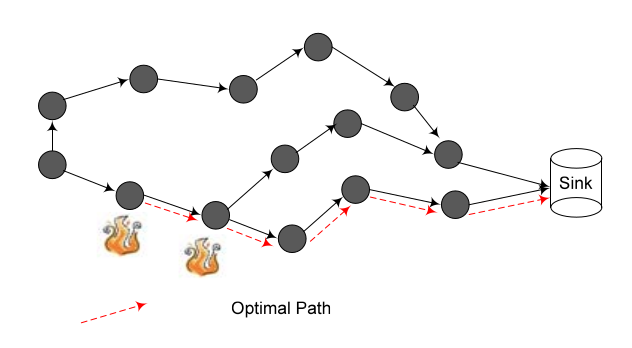
\includegraphics[scale=0.35]{img/network.png}
    \caption{Energy-efficient data forwarding in wireless sensor networks\cite{WSN2014}}
    \label{figex_network}
\end{figure}
The Energy associated with sensor nodes is constantly changing as packets are received by that node, thus modifying the edge weights of the network. So after each round, A* is performed to find the energy-efficient path to the Base station. Our algorithm can eliminate applying A* again and again, as we can simulate the weight change as deletion of that edge and then insertion of the same edge with the new weight. To show this and evaluate the performance gain we implemented EERP~\cite{WSN2014} and instead of doing repeated A* we used our DA* to find the optimal path.\\

In EERP~\cite{WSN2014} author proposed a scheme where the value of
function $f(x)$ is equal to the node cost of node n, and the intention is to forward data packets to the next neighbor node which has higher residual energy, higher free buffer, and higher packet reception rate. To achieve this, they made use of the aggregated weight of the above-mentioned routing parameters. They define the aggregated weight of a next neighbor node as the sum of normalized weights of its routing metrics as follows:
\begin{equation}
    g(n) = \text{Min}(\alpha(\frac{E_{ini}(n)}{E_{res}(n}) + \beta(\frac{N_t(n)}{N_r(n)}) + \gamma(\frac{B_{ini}(n)}{B_f(n)}) )
\end{equation}

Where $E_{res}(n)$ and $E_{ini}(n)$ are residual and initial energy of node n respectively, $N_r(n)$ and $N_t(n)$  are the number of transmitted and received packets respectively, $B_f(n)$ and $B_{ini}(n)$ referred to the number of free and initial buffer of node $n$ respectively, $\alpha$, $\beta$ and $\gamma$ are weight parameters and $\alpha + \beta + \gamma = 1$.\\
And the value of $h(n)$ function can be calculated as:
\begin{equation}
h(n) = \frac{d(n,s)}{\text{avg}(d(n,j))}
\end{equation} Where $d(n,s)$ is the distance between the node and sink node and $a\text{vg}(d(n,j))$ is the average distance between the node $n$ and its one hop neighbouring nodes$(j)$.\\
To build the routing table authors\cite{WSN2011} proposed algorithm where A* is performed for each node to find the best path to sink, after each round.
% \newpage
\begin{lstlisting} [language=C, caption=Pseudo Code for Proposed Efficient Routing Algorithm\cite{WSN2011}]
Input: Sensor Network
Output : Life of Sensor Network in terms of rounds
BEGIN
    InitilizeNetwork()
    EstimateDistance()              // finds distance to the sink
    WHILE NOT END_ASTAR()           // N-of-N metric [11]
        InitializeSolArray()        // initialize solution
                                    //array to store routing schedule
        FOR each node i in the Network DO
            CreateTree (i)          //using A-Star algorithm
            PrepareSolArray()       //prepare routing schedule
        END FOR
        BroadcastSolution()        // BS broadcasts routing schedule
        UpdateEnergy()               //Energy update for relay nodes
        CountRound = CountRound + 1  //count n/w life
    END WHILE
    PRINT CountRound                //print n/w lifetime in
END
\end{lstlisting}
Instead of performing A* for each node to find the path, we take the idea from D*~\cite{original_D_star} where to find the path the search starts from the destination node towards the source node. So to find paths to all nodes our we start A* from sink node and end when we have visited all nodes. After BroadCastSolution() we UpdateEnergy() and then add all those edges to update\_list whose weights are modified and then on it we apply our propagation methods described in the above sections to find the optimal\_path and thus forming new routing table at the base station.

\begin{lstlisting}[language=C, caption=EERP with DA*, label=WSNDA]
Input: Sensor Network
Output: Life of Sensor Network in terms of rounds
BEGIN
    InitilizeNetwork()
    EstimateDistance()          // finds distance to the sink
    InitializeSolArray()         //array to store routing schedule
    
    ASTAR_From_Sink()          //finds path to all nodes from sink
    BroadcastSolution()        // BS broadcasts routing schedule
    UpdateEnergy()               //Energy update for relay nodes
    CountRound = CountRound + 1
    
    WHILE NOT END_ASTAR()
        Create_UpdateList()   //list of edges whose weight is changed
        Propagation()         //Propagate change using methods of DA*  
        Update_SolArray()     //Update routing table with new path
        BroadcastSolution()         // BS broadcasts routing schedule
        UpdateEnergy()             //Energy update for relay nodes
        CountRound = CountRound + 1
    END WHILE
    PRINT CountRound                //print n/w lifetime 
END
\end{lstlisting}
The energy consumption model of the EERP~\cite{WSN2014}, the authors used the first order radio model which is the typical model in the area of routing protocol evaluation in WSN~\cite{WSN_energy}. According to this model, the energy consumed for transmitting and receiving k-bit data can be calculated as follows~\cite{WSN_energy}:
\begin{align*}
    E_{Tx}(k) &= k (E_{elec} + \epsilon_{amp}.d^2) \\
    E_{Rx}(k) &= k.E_{elec} \\
    E_T(k) &= E_{Tx}(k) + E_{Rx}(k) = k(2E_{elec} +\epsilon_{amp}.d^2)
\end{align*}
Here we compare the life expectancy of network and performance of algorithms EERP~\cite{WSN2014}, A~*\cite{A*}, DA* for routing the packets in WSN. All algorithms are implemented in CUDA and ran on Tesla K40c a keepler based GPU with 15 SMs and 192 SP per SM for a total of 2880 SPs.
\begin{figure}[H]
    \centering
    \begin{subfigure}[b]{0.47\textwidth}
         \centering
         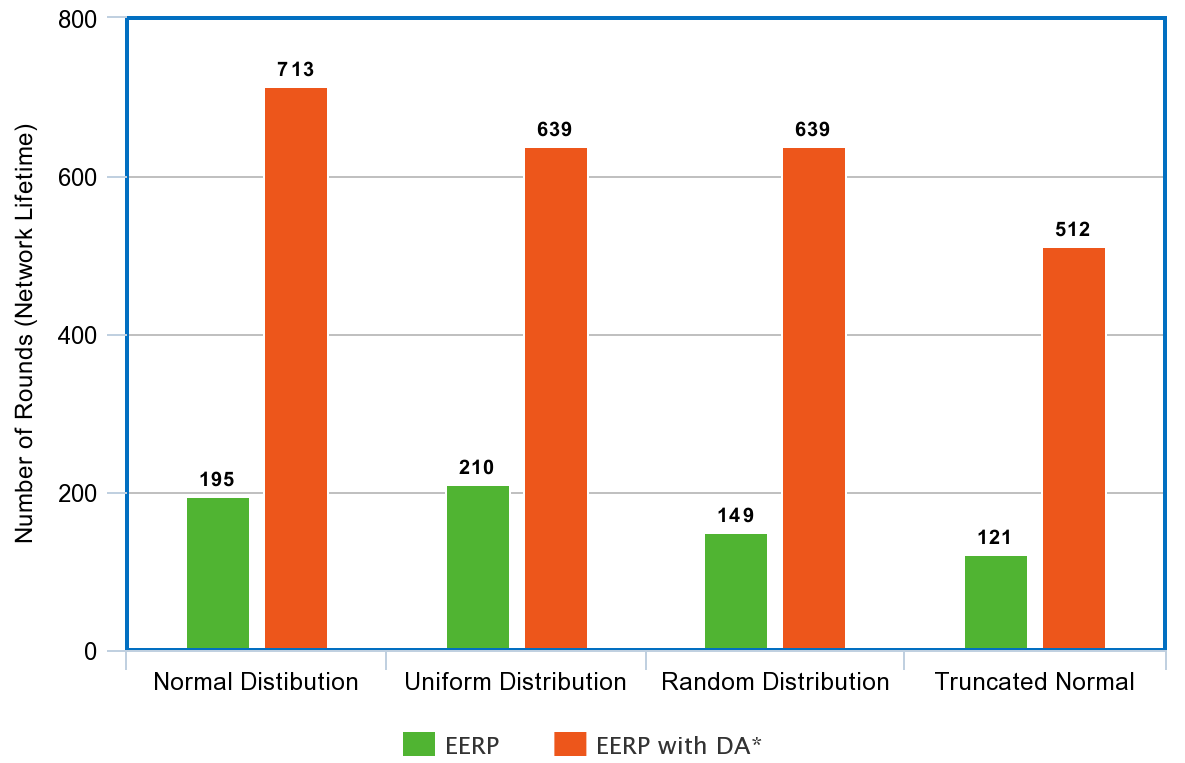
\includegraphics[width=\textwidth]{img/chart.png}
         \caption{Network Lifetime Comparison }
         \label{fig:wsn_life}
    \end{subfigure}
    \hfill
    \begin{subfigure}[b]{0.47\textwidth}
        \centering
         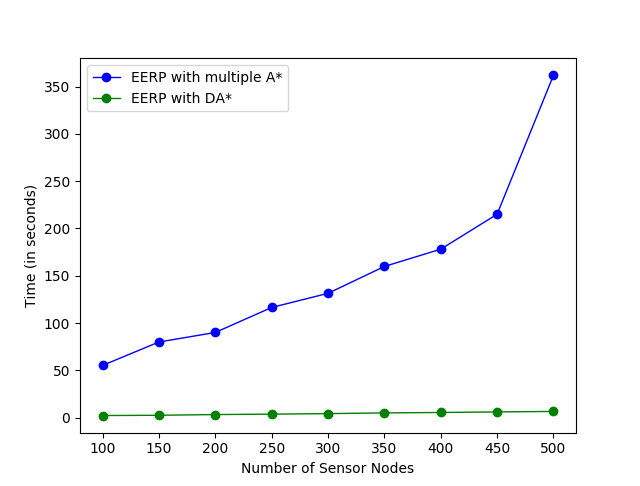
\includegraphics[width=\textwidth]{img/eerp.png}
         \caption{Execution Time vs Number of Nodes}
         \label{fig:wsn_runtime}
    \end{subfigure}
    \caption{}
    \label{fig:wsn_plots}
\end{figure}
\todo{Error in bar plot naming }
In Figure~\ref{fig:wsn_life} we compare A* routing algorithm with EERP~\cite{WSN2014} with different node (sensor node) distribution. For all the distributions we have taken that sensor nodes area dispersed in are of 100x100 $m^2$, and the base station is located at coordinate (50,50), and the number of nodes is 150 with each having range of 20m. EERP increases the network lifetime by almost 3x in each distribution. Most of the real-world networks follow a normal distribution as more sensor nodes are concentrated near the base station (sink). The Figure~\ref{fig:wsn_runtime} shows how the execution time of EERP is boosted by using our algorithm, For 100 nodes in network, we get 24x speedup, as the number of nodes in network increases the execution time of EERP increases much faster than EERP with DA*, with 500 nodes we get 55x speedup. Its because our algorithm scales well wrt the number of updates (here number of rounds) and size of graph compared to repeating A*, as we only update the parts of the graph which are affected by the change.  

%\subsection{Path Finding and Mazes}


\section{Related Work}\label{sec:related_work}
A*~\cite{A*} is one of the widely used path-finding algorithms, Peter Hart, Nils Nilsson and Bertram Raphael of Stanford Research Institute (now SRI International) first published the algorithm in 1968. It can be seen as an extension of Dijkstra's algorithm where $h(x)=0 $ $\forall x, x \in V$. A* achieves better performance by using heuristics to guide its search. What makes it different from the greedy best-first algorithm is it takes already traveled distance $g(x)$ into account.

D*~\cite{original_D_star}, focused D*~\cite{focused_D_star} and D* lite~\cite{D_star_lite} are a family of incremental search algorithms. The original D*~\cite{original_D_star} by Anthony Stentz is an informed incremental search algorithm. Focused D*\cite{focused_D_star} is an informed incremental heuristic search algorithm by Anthony Stentz that combines ideas of A*~\cite{A*} and the original D*\cite{original_D_star}. Focused D* resulted from further development of the original D*. D* Lite~\cite{D_star_lite} is an incremental heuristic search algorithm by Sven Koenig and Maxim Likhachev that builds on LPA*~\cite{LPA*}, an incremental heuristic search algorithm that combines ideas of A* and Dynamic SWSF-FP~\cite{SPP}. All three search algorithms solve the same assumption-based path planning problems, including planning with the free space assumption~\cite{PF} where a robot has to navigate to given goal coordinates in unknown terrain. So in all the three algorithms, the graph is changing while we try to find the shortest path to the destination, this is a major difference between our algorithm and D* as we try to find the shortest path to destination after some changes(insertion + deletion) has occurred since our last search. Another major change is in D* only the cost of edges is changed while the number of edges remains fixed But in our case edges can be removed as well as added and the cost change can be emulated as deleting that edge and later adding the same edge with the new cost. The name D* comes from the term "Dynamic A*" because the algorithm behaves like A* except that the arc costs can change as the algorithm runs.

\section{Conclusion and Future Work}\label{sec:future_work}
We have proposed an algorithm that can efficiently find the optimal path with the help of heuristics on GPU while taking account of updates in the form of insertion and deletions with time. Our algorithm is faster than doing repeated A* on GPU from scratch. We also found that insertions take less time to process than deletion. And due to the fact that both insertion and deletion requires a different set of instruction to process, separate propagation outperforms simultaneous propagation.

In the future, the possibility of Dynamic A* in a multi-GPU environment can also be explored. There can be algorithmic development in dynamic bi-directional A* on GPU. A* is used in a wide variety of applications and many such applications are based on graphs that are dynamic in nature. In the future, many such applications like maze solver, SCPR (structural based computational protein design) and codon optimization can be modified to use DA* to boost their performance.

\printbibliography
%\newpage
% %\newpage 
%     \section{Appendix} 
%     \subsection{Heuristics in A*}
%      Performance of A* depends heavily on the type of heuristics that are used. It guides the search to reach the destination faster, but wrong values can also lead to slower or a path that is not the shortest path.
%      $\forall x \in V$
%      \begin{itemize}
%          \item If $h(x)=0$, then A* turns into in Dijkstra's Algorithm.
%          \item If $h(x) \leq$ cost of reaching destination from x, We are guaranteed to find the shortest path but it will be slower.
%          \item If $h(x) = $cost of reaching destination from x, we will follow only the best path.
%          \item If $h(x)$ is sometimes greater than cost of reaching destination from $x$. A* is not guaranteed to find the shortest path.
%          \item If $h(x)>> g(x)$, then only $h(x)$ plays a role and A* turns into greedy best first search.
%      \end{itemize}
%     Considering the above factors in our implementation for general graphs we chose $h(x)$ as bfs distance from destination to $x$, so we are always guaranteed to find the shortest path.
%     % \subsection{Storing dynamic Graph on GPU}
%     % \subsection{Global Lock in GPU}
    

% Lockin implementation, K PQ implemetation, GA* implementation

\end{document}